% =================================================================== %
%   Tesis (template)
% =================================================================== %
%
%\documentclass[12pt,twoside,draft]{book}
\documentclass[12pt,twoside]{book}

% la opci�n draft es bueno activarla mientras uno est� escribiendo y despu�s hay que sacarla para la versi�n final 

% packages LaTeX adicionales
\usepackage[spanish]{babel}
\usepackage{amsmath}
\usepackage{amstext}
\usepackage{amssymb}
\usepackage{longtable}
\usepackage{makeidx}
\usepackage[dvips]{graphicx}


\def\setbmp#1#2#3#4{\vskip#3\relax\noindent\hskip#1\relax
 \special{bmp:#4 x=#2, y=#3}}
\def\centerbmp#1#2#3{\vskip#2\relax\centerline{\hbox to#1{\special
  {bmp:#3 x=#1, y=#2}\hfil}}}


% idioma espa�ol
\selectlanguage{spanish}

% m�rgenes
\setlength{\textwidth}{150mm}
\setlength{\oddsidemargin}{9.6mm}
\setlength{\evensidemargin}{-0.6mm}
\setlength{\textheight}{217mm}
\setlength{\topmargin}{-5.4mm}
\setlength{\headheight}{10mm}
\setlength{\headsep}{10mm}

% doble espaciado entre lineas
\def\baselinestretch{1.30}

% profundidad en la tabla de contenidos
\setcounter{tocdepth}{4}

% hasta donde pone n�meros en el seccionado (ej 1.3.4.1)
\setcounter{secnumdepth}{4}

% definiciones de comandos especiales
%--------------------------------------------------------------------------
% Comandos usados en la tesis
%--------------------------------------------------------------------------


%--------------------------------------------------------------------------
% Definiciones de ambientes
%--------------------------------------------------------------------------
\newtheorem{defx}{Definici\'on}[chapter]
\newtheorem{lemx}{Lema}[chapter]
\newtheorem{corox}{Corolario}[chapter]
\newtheorem{algx}{Algoritmo}[chapter]
\newtheorem{ejemx}{Ejemplo}[chapter]
\newtheorem{propx}{Proposici\'on}[chapter]
\newtheorem{teox}{Teorema}[chapter]
\newtheorem{obsx}{Observaci\'on}[chapter]


\newenvironment{defi}[1]
    {\begin{defx}\rm(\emph{#1})\\}
    {\hfill $\blacksquare$ \end{defx}}

\newenvironment{ejem}
    {\begin{ejemx}\setlength{\parindent}{0pt}\rm}
    {\hfill $\blacksquare$ \end{ejemx}}

\newenvironment{alg}
    {\begin{algx}\begin{rm}}
    {\noindent \end{rm}\end{algx}}

\newenvironment{dem}
    {\textbf{Demostraci\'on:} \rm}
    {\hfill $\square$}\medskip

\newenvironment{lema}
    {\begin{lemx}\rm}
    {\hfill $\blacksquare$ \end{lemx}}

\newenvironment{obser}
    {\begin{obsx}\rm}
    {\hfill $\blacksquare$ \end{obsx}}

\newenvironment{prop}
    {\begin{propx}\rm}
    {\hfill $\blacksquare$ \end{propx}}

\newenvironment{coro}
    {\begin{corox}\rm}
    {\hfill $\blacksquare$ \end{corox}}

\newenvironment{teo}
    {\begin{teox}\rm}
    {\hfill $\blacksquare$ \end{teox}}

\newenvironment{obs}
    {\noindent {\textsc{Observaci\'on:\ }}}
    {}

%--------------------------------------------------------------------------
% Algunas siglas
%--------------------------------------------------------------------------
\newcommand{\TMS}{{\small TMS}}
\newcommand{\MTDR}{{\small MTDR}}
\newcommand{\PLR}{{\small PLR}}
\newcommand{\PLRO}{{\small PLRO}}
\newcommand{\SAA}{{\small SAA}}
\newcommand{\OSCAR}{{\small OSCAR}}
%--------------------------------------------------------------------------
% Comandos �tiles
%--------------------------------------------------------------------------

\newcommand{\tab}{\hspace*{1cm}}
\newcommand{\true}{\mbox{\textsc{true}}}
\newcommand{\false}{\mbox{\textsc{false}}}


\makeindex
% =================================================================== %

\begin{document}

\nocite{*}

\frontmatter\pagestyle{empty}

\begin{titlepage}
\begin{titlepage}

\begin{center}

\includegraphics[width=3cm,height=3cm]{uni.png}
\end{center}

\begin{center}

\textbf{\LARGE Universidad Nacional del Sur}\\

\vspace{2cm}

\textsc{\LARGE Proyecto Final de Carrera}\\ \vspace{.1cm}
\textsc{\LARGE Ingenier\'ia en Computaci\'on}\\


\vspace{4cm}

\emph{\LARGE Seguridad en redes LAN: utilizando Docker para mejorar la navegación web.}\\

\vspace{2.5cm}

{\Large Salvador Catalfamo}\\

\vspace{2.5cm}

{\sc\Large Bah\'{\i}a Blanca -- Argentina}\\
\vspace*{.1cm} {\Large 2021}

\end{center}
\end{titlepage}

\end{titlepage}

\begin{titlepage}
\begin{titlepage}

\begin{center}

\includegraphics[width=3cm,height=3cm]{uni.png}
\end{center}

\begin{center}

\textbf{\LARGE Universidad Nacional del Sur}\\

\vspace{2cm}

\textsc{\LARGE Proyecto Final de Carrera}\\ \vspace{.1cm}
\textsc{\LARGE Ingenier\'ia en Computaci\'on}\\


\vspace{4cm}

\emph{\LARGE Seguridad en redes LAN: utilizando Docker para mejorar la navegación web.}\\

\vspace{2.5cm}

{\Large Salvador Catalfamo}\\

\vspace{2.5cm}

{\sc\Large Bah\'{\i}a Blanca -- Argentina}\\
\vspace*{.1cm} {\Large 2021}

\end{center}
\end{titlepage}

\end{titlepage}


% =================================================================== %

\setcounter{page}{1}

% resumen en castellano
\thispagestyle{empty}
\chapter*{Resumen}

% Aca va el resumen en castellano

\bigskip
A lo largo de la carrera, hemos visto como las organizaciones abordan los temas de seguridad en sus sistemas informáticos. Mayormente, se concentran en los equipos que están expuestos a la red pública, dejando de lado los que se encuentran aislados de la misma. Erróneamente, muchas veces se piensa que es suficiente, sin embargo, puede traer graves inconvenientes. Es por eso que realizaremos un estudio teórico/práctico sobre las consecuencias de la navegación en redes internas sin ningún tipo de cifrado de datos ni certificaciones.

\bigskip
\noindent \textsc{Palabras Clave:} \par

Seguridad e Infraestructura\par
Docker \par
Linux \par
Kali \par
Máquinas Virtuales  \par




\tableofcontents

%\listoffigures

% =================================================================== %
\mainmatter\pagestyle{headings}


\chapter{Introducci\'on} \setcounter{page}{1}\pagenumbering{arabic}
    \label{capIntro}

%-*- ES -*-
%----------------------------------------------------------------------
% capitulo 1: Introduccion
%----------------------------------------------------------------------
% Estructura del capitulo:
%
%----------------------------------------------------------------------


% se pone una introducci�n al tema en general

\section{Objetivos}

\begin{itemize}
 \item item 1
 \item item 2
\end{itemize}


\begin{verbatim}
 Este es un bien ambiente para 
poner codigo
\end{verbatim}



En \cite{Davis:1989} se \footnote{Esta es una nota al pie} ve...
\\
\textit{casa} \\
\emph{casa} \\
\texttt{casa} \\
\textsf{casa} \\
\textbf{casa} \\

\subsection{objetivos principales}

\subsubsection{particulares}

\begin{center}
\begin{figure}


\includegraphics[width=3cm,height=3cm]{uni.bmp}

\caption{Esta es la figura del escudo de la uns}
\end{figure}
\end{center}

\section{Plan de tesis y principales contribuciones}\label{secContribuciones}

\section{Trabajos previos relacionados}
% rese�ar los art�culos hechos en el contexto del trabajo de tesis si los hay



% =================================================================== %

\chapter{Descripci\'on del problema} \setcounter{page}{1}\pagenumbering{arabic}
    \label{capDesc}

%-*- ES -*-
%----------------------------------------------------------------------
% Capitulo 7: Descripción del problema

En éste capítulo se verá por qué los protocolos http y smtp son inseguros, introducción al snnifin, spoofing, arp attack
%----------------------------------------------------------------------

(Agregar una intro)

\section{Establishing Authority}

HTTP relies on the notion of an authoritative response: a response
that has been determined by (or at the direction of) the authority
identified within the target URI to be the most appropriate response
for that request given the state of the target resource at the time
of response message origination.  Providing a response from a
non-authoritative source, such as a shared cache, is often useful to
improve performance and availability, but only to the extent that the
source can be trusted or the distrusted response can be safely used.

Unfortunately, establishing authority can be difficult.  For example,
phishing is an attack on the user's perception of authority, where
that perception can be misled by presenting similar branding in
hypertext, possibly aided by userinfo obfuscating the authority
component (see Section 2.7.1).  User agents can reduce the impact of
phishing attacks by enabling users to easily inspect a target URI
prior to making an action, by prominently distinguishing (or
rejecting) userinfo when present, and by not sending stored
credentials and cookies when the referring document is from an
unknown or untrusted source.

When a registered name is used in the authority component, the "http"
URI scheme (Section 2.7.1) relies on the user's local name resolution
service to determine where it can find authoritative responses.  This
means that any attack on a user's network host table, cached names,
or name resolution libraries becomes an avenue for attack on
establishing authority.  Likewise, the user's choice of server for
Domain Name Service (DNS), and the hierarchy of servers from which it
obtains resolution results, could impact the authenticity of address
mappings; DNS Security Extensions are one way to
improve authenticity.

Furthermore, after an IP address is obtained, establishing authority
for an "http" URI is vulnerable to attacks on Internet Protocol
routing.


\section{Risks of Intermediaries}

By their very nature, HTTP intermediaries are men-in-the-middle and,
thus, represent an opportunity for man-in-the-middle attacks.
Compromise of the systems on which the intermediaries run can result
in serious security and privacy problems.  Intermediaries might have
access to security-related information, personal information about
individual users and organizations, and proprietary information
belonging to users and content providers.  A compromised
intermediary, or an intermediary implemented or configured without
regard to security and privacy considerations, might be used in the
commission of a wide range of potential attacks.

Intermediaries that contain a shared cache are especially vulnerable
to cache poisoning attacks.
Implementers need to consider the privacy and security implications
of their design and coding decisions, and of the configuration
options they provide to operators (especially the default
configuration).

Users need to be aware that intermediaries are no more trustworthy
than the people who run them; HTTP itself cannot solve this problem.

\section{Attacks via Protocol Element Length}

Because HTTP uses mostly textual, character-delimited fields, parsers
are often vulnerable to attacks based on sending very long (or very
slow) streams of data, particularly where an implementation is
expecting a protocol element with no predefined length.



\section{Response Splitting}

Response splitting (a.k.a, CRLF injection) is a common technique,
used in various attacks on Web usage, that exploits the line-based
nature of HTTP message framing and the ordered association of
requests to responses on persistent connections [Klein].  This
technique can be particularly damaging when the requests pass through
a shared cache.

Response splitting exploits a vulnerability in servers (usually
within an application server) where an attacker can send encoded data
within some parameter of the request that is later decoded and echoed
within any of the response header fields of the response.  If the
decoded data is crafted to look like the response has ended and a
subsequent response has begun, the response has been split and the
content within the apparent second response is controlled by the
attacker.  The attacker can then make any other request on the same
persistent connection and trick the recipients (including
intermediaries) into believing that the second half of the split is
an authoritative answer to the second request.

For example, a parameter within the request-target might be read by
an application server and reused within a redirect, resulting in the
same parameter being echoed in the Location header field of the
response.  If the parameter is decoded by the application and not
properly encoded when placed in the response field, the attacker can
send encoded CRLF octets and other content that will make the
application's single response look like two or more responses.


\section{Request Smuggling}

Request smuggling ([Linhart]) is a technique that exploits
differences in protocol parsing among various recipients to hide
additional requests (which might otherwise be blocked or disabled by
policy) within an apparently harmless request.  Like response
splitting, request smuggling can lead to a variety of attacks on HTTP
usage.


\section{Message Integrity}

HTTP does not define a specific mechanism for ensuring message
integrity, instead relying on the error-detection ability of
underlying transport protocols and the use of length or
chunk-delimited framing to detect completeness.  Additional integrity
mechanisms, such as hash functions or digital signatures applied to
the content, can be selectively added to messages via extensible
metadata header fields.  Historically, the lack of a single integrity
mechanism has been justified by the informal nature of most HTTP
communication.  However, the prevalence of HTTP as an information
access mechanism has resulted in its increasing use within
environments where verification of message integrity is crucial.

User agents are encouraged to implement configurable means for
detecting and reporting failures of message integrity such that those
means can be enabled within environments for which integrity is
necessary.  For example, a browser being used to view medical history
or drug interaction information needs to indicate to the user when
such information is detected by the protocol to be incomplete,
expired, or corrupted during transfer.  Such mechanisms might be
selectively enabled via user agent extensions or the presence of
message integrity metadata in a response.  At a minimum, user agents
ought to provide some indication that allows a user to distinguish
between a complete and incomplete response message (Section 3.4) when
such verification is desired.

\section{Message Confidentiality}

HTTP relies on underlying transport protocols to provide message
confidentiality when that is desired.  HTTP has been specifically
designed to be independent of the transport protocol, such that it
can be used over many different forms of encrypted connection, with
the selection of such transports being identified by the choice of
URI scheme or within user agent configuration.

\section{Tipes of Attacks}
There are mainly two types of network attacks – passive attack and active attack

Passive: This type of attack happens when sensitive information is monitored and
analyzed, possibly compromising the security of enterprises and their customers.
In short, network intruder intercepts data traveling through the network.
• Active: This type of attack happens when information is modified, altered or
demolished entirely by a hacker. Here the interloper starts instructions to disturb
the network’s regular process.

So the motives behind passive attackers and active attackers are totally different.
Whereas the motive of passive attackers is simply to steal sensitive information and
to analyze the traffic to steal future messages, the motive of active attackers is to stop
normal communication between two legitimate entities.
\subsection{Passive Attacks}
Passive attackers aremainly interested in stealing sensitive information. This happens
without the knowledge of the victim. As such passive attacks are difficult to detect
and thereby secure the network. The following are some of the passive attacks that
are in existence [7].
\begin{itemize}
    \item Traffic Analysis: Attacker senses the communication path between the sender
    and receiver.
    \item Monitoring: Attacker can read the confidential data, but he cannot edit or modify
    the data.
    \item Eavesdropping: This type of attack occurs in the mobile ad-hoc network where
    basically the attacker finds out some secret or confidential information from
    communication.
\end{itemize}

\subsection{Active Attacks}
The active attacks happen in such a manner so as to notify the victims that their
systems have been compromised. As a result, the victim stops communication with
the other party. Some of the active attacks are as follows [8].
\begin{itemize}
    \item Modification: Some alterations in the routing route is performed by the malicious
    node. This results in causing the sender to send messages through the long route,
    which causes communication delay. This is an attack on integrity as shown in
    Fig. 2.
    \item Wormhole: This attack is also called a tunneling attack. A packet is received
    by an attacker at one point. He then tunnels it to another malicious node in the
    network. This causes a beginner to assume that he found the shortest path in the
    network as shown in Fig. 3.
    \item Fabrication: A malicious node generates a false routing message that causes the
    generation of incorrect information about the route between devices. This is an
    attack on authenticity as shown in Fig. 4.    
    \item Spoofing: A malicious node miss-present his identity so that the sender changes
    his topology as shown in Fig. 5.
    \item Denial of services: A malicious node sends a message to the node and consumes
    the bandwidth of the network as given in Fig.
    \item  Man-in-the-middle: Attack—Also called a hijacking attack, it is an attack where
    the attacker secretly alters and relays the communications between two legitimate
    parties without their knowledge. These parties in turn are unaware of the secret
    hacker consider that they are doing direct communication with each other [13].
    Figure 12 depicts this attack.
\end{itemize}

\section{Caso de estudio: Sniffing de la red para obtener credenciales}

\subsection{Herramienta Utilizadas} 
    

\subsubsection*{Kali Linux}
Kali Linux es una distribución de Linux (basada en Debian) centrada en la seguridad. 
Es una versión renombrada de la famosa distribución de Linux conocida como Backtrack, 
que venía con un enorme repositorio de herramientas de piratería de código abierto, 
para pruebas de penetración de aplicaciones \emph{web}, inalámbricas y de red. 

\begin{center}
    \begin{figure}   
       \begin{center}
          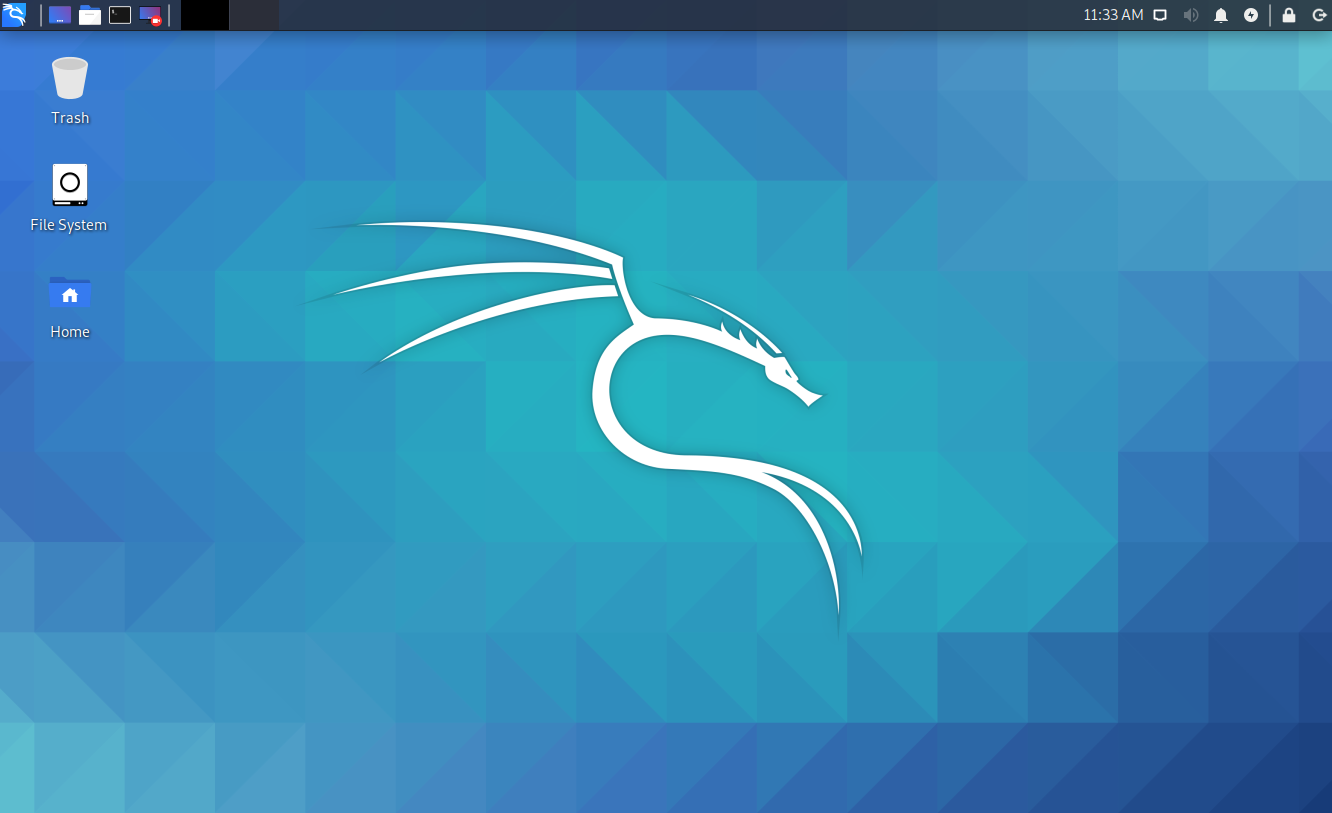
\includegraphics[width=11cm,height=7cm]{ataque-1.png}
       \end{center}
       \caption{Escritorio de Kali Linux}
    \end{figure}
 \end{center}
 

Kali Linux contiene muchas herramientas preinstaladas con 
todas las dependencias y ya está lista para usar. Esto nos permite tener que prestar 
más atención a las pruebas y no a la instalación de la herramienta. Las actualizaciones 
para las herramientas instaladas en Kali Linux se publican con mayor frecuencia, 
lo que le ayuda a mantener las a las mismas actualizadas.

Esta distribución contiene las herramientas necesarias para realizar nuestro
ataque.

\subsubsection*{Wireshark}
Wireshark es uno de los analizadores de protocolos de red más populares, es de 
código abierto y gratuito. Wireshark está preinstalado en Kali y es ideal para la 
resolución de problemas de red, análisis y, para este caso de estudio, una herramienta 
perfecta para monitorear el tráfico de posibles objetivos. Wireshark usa un kit de 
herramientas para implementar su interfaz de usuario y para capturar paquetes. 
Funciona de manera muy similar a un comando \emph{tcpdump}; sin embargo, nos brinda
una interfaz gráfica, posee opciones integradas de clasificación y filtrado.

\begin{center}
    \begin{figure}   
       \begin{center}
          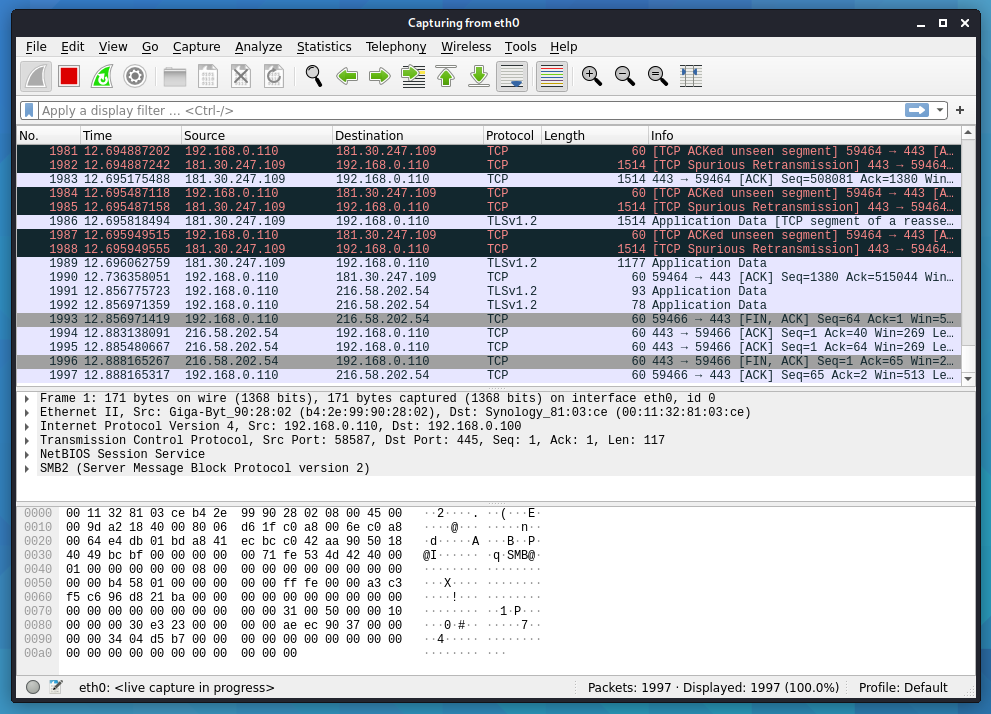
\includegraphics[width=10cm,height=7cm]{wireshark.png}
       \end{center}
       \caption{Interface del Wireshark}
    \end{figure}
 \end{center}
 
\subsubsection*{Ettercap}

\begin{center}
   \begin{figure}   
      \begin{center}
         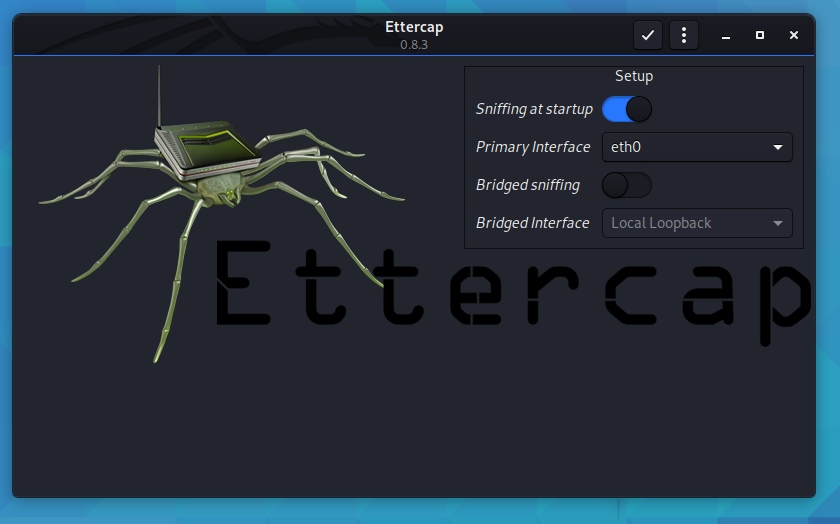
\includegraphics[width=10 cm,height=7cm]{ataque-2.png}
      \end{center}
      \caption{Ettercap}
   \end{figure}
\end{center}

Ettercap es un paquete completo gratuito y de código abierto para ataques basados 
en intermediarios. Ettercap se puede utilizar para análisis de protocolos de redes 
informáticas y auditorías de seguridad, con funciones de rastreo de conexiones en 
tiempo real y filtrado de contenido. Ettercap funciona configurando la interfaz de red 
del atacante en modo promiscuo y \emph{ARP} para envenenar las máquinas víctimas.



\subsection{Realización del ataque}

\begin{center}
    \begin{figure}   
       \begin{center}
          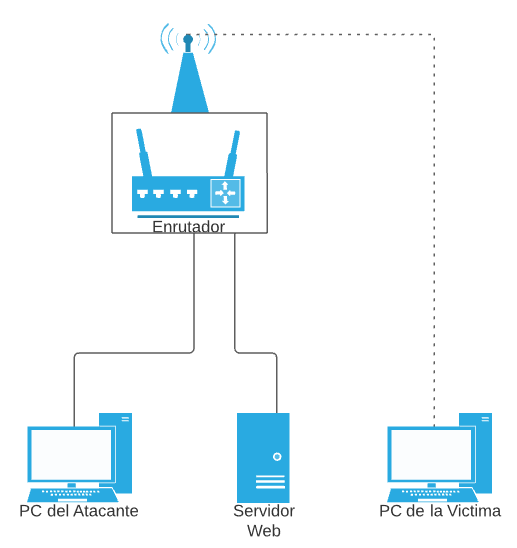
\includegraphics[width=9cm,height=9cm]{red.png}
       \end{center}
       \caption{Escenario montado}
    \end{figure}
 \end{center}

La idea principal de esta sección es demostrar que, encontrándose en una red interna
y con herramientas ya desarrolladas y libres, es posible realizar un ataque 
sin necesidad de conocer a fondo la implementación de la misma ni de tener mayores
privilegios.

El escenario consiste en crear una página web con un 
simple formulario donde se debe completar con usuario y contraseña, y un 
submit el cual envía esta información desde el cliente hasta el 
servidor web. El envío de este formulario contiene la información confidencial,
 por lo que en un escenario seguro ningún
intermediario podría obtener estos datos. Dado que este tráfico va a 
circular por HTTP, demostraremos como nos podemos hacer de las credenciales
ingresadas por el usuario.

\begin{center}
   \begin{figure}   
      \begin{center}
         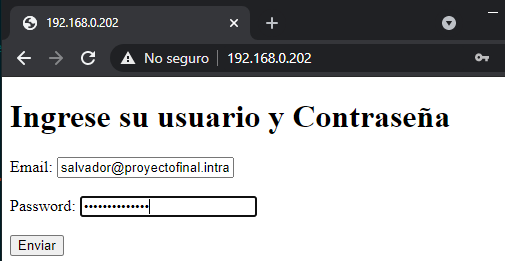
\includegraphics[width=10cm,height=6cm]{form.png}
      \end{center}
      \caption{Formulario montado}
   \end{figure}
\end{center}

Recordar que esto fue realizado en una red interna donde son todos equipos de nuestra propiedad.


\subsection{Preparando Ettercap para el ataque ARP Poisoning}

Lo primero que debemos hacer, en la lista de aplicaciones, es buscar el apartado 
\emph{Sniffing} y \emph{Spoofing}, ya que es allí donde encontraremos las herramientas necesarias
 para llevar a cabo este ataque. A continuación, abriremos Ettercap.

\begin{center}
    \begin{figure}   
       \begin{center}
          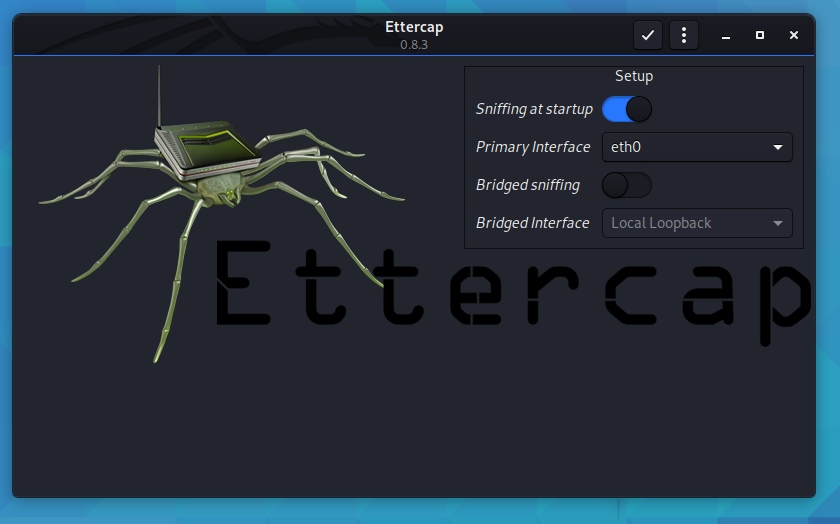
\includegraphics[width=9 cm,height=6cm]{ataque-2.png}
       \end{center}
       \caption{Ettercap}
    \end{figure}
 \end{center}

El siguiente paso es seleccionar la tarjeta de red con la que vamos a trabajar. Para 
ello, en el menú superior de Ettercap seleccionaremos Sniff $>$ Unified Sniffing y, 
cuando nos lo pregunte, seleccionaremos nuestra tarjeta de red (por ejemplo, en 
nuestro caso, eth0).

Luego se debe buscar todos los hosts conectados a nuestra red local. Para ello, 
seleccionaremos Hosts del menú de la parte superior y seleccionaremos la primera 
opción, Hosts List.

Allí deberían salirnos todos los hosts o dispositivos conectados a nuestra red. 
Sin embargo, en caso de que no salgan todos, podemos realizar una exploración 
completa de la red simplemente abriendo el menú Hosts y seleccionando la opción 
Scan for hosts. Tras unos segundos, la lista de antes se debería actualizar 
mostrando todos los dispositivos, con sus respectivas IPs y MACs, conectados 
a nuestra red.



\subsection{Nuestro Ettercap ya está listo. Ya podemos empezar con el ataque ARP Poisoning}

En caso de querer realizar un ataque dirigido contra un solo host, por ejemplo, 
suplantar la identidad de la puerta de enlace para monitorear las conexiones 
de la víctima, antes de empezar con el 
ataque debemos establecer los dos objetivos.

Para ello, debajo de la lista de hosts podemos ver tres botones, aunque nosotros 
prestaremos atención a los dos últimos:

    Target 1 – Seleccionamos la IP del dispositivo a monitorear, en este caso, 
    la computadora de la víctima, y pulsamos sobre dicho botón.

    Target 2 – Pulsamos la IP que queremos suplantar, en este caso, la de la 
    puerta de enlace y la del servidor web.

    \begin{center}
        \begin{figure}   
           \begin{center}
              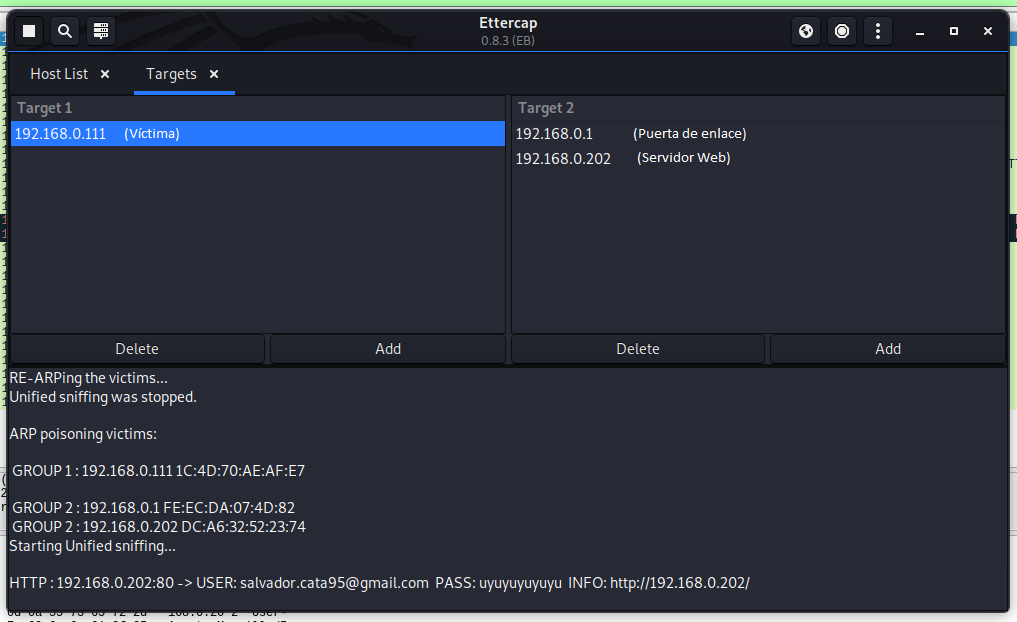
\includegraphics[width=17cm,height=9.5cm]{ataque-7-deta.png}
           \end{center}
           \caption{Ettercap}
        \end{figure}
     \end{center}

Todo listo. Ahora solo debemos elegir el menú MITM de la parte superior y, en él, 
escoger la opción ARP Poisoning. Nos aparecerá una pequeña ventana de configuración, 
en la cual debemos asegurarnos de marcar Sniff Remote Connections.
Pulsamos sobre Ok y el ataque dará lugar. Ahora ya podemos tener el control 
sobre el host que hayamos establecido como Target 1. Lo siguiente que debemos 
hacer es, ejecutar Wireshark para capturar todos los paquetes de 
red y analizarlos en busca de información interesante.

\begin{center}
   \begin{figure}   
      \begin{center}
         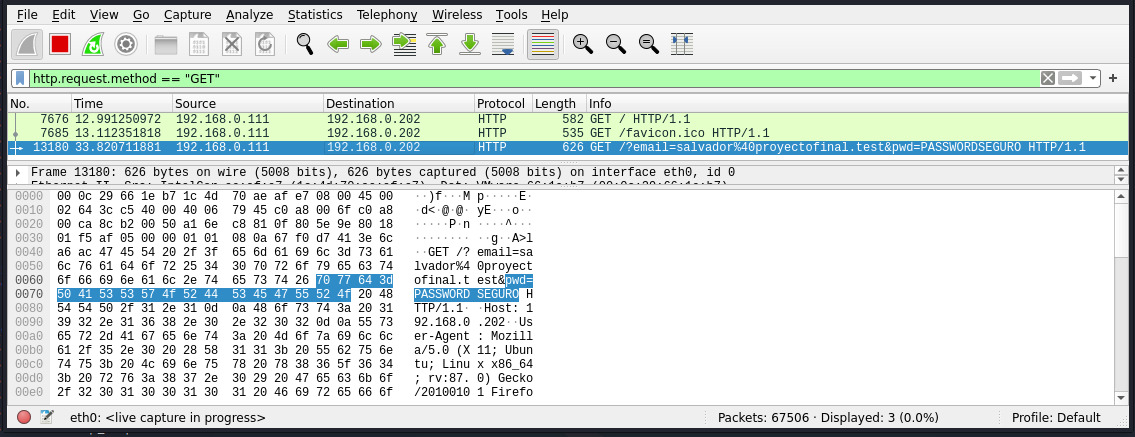
\includegraphics[width=17cm,height=7cm]{paquetes.png}
      \end{center}
      \caption{Paquetes capturados}
   \end{figure}
\end{center}

Como se puede ver, Wireshark nos permite filtrar el tráfico, y con el 
simple hecho de decirle que queremos mostrar los requerimientos GET
pudimos dar con el paquete que queríamos, en el request podemos ver
el usuario “salvador@proyectofinal.test” y la contraseña “PASSWORD SEGURO”




\chapter{Implementaci\'on de la soluci\'on propuesta} \setcounter{page}{1}\pagenumbering{arabic}
    \label{capImp}

%-*- ES -*-
%----------------------------------------------------------------------
% Capitulo: Implementacion de la solución propuesta
%----------------------------------------------------------------------

\section{Propuestas: Introducción}

Se han investigado tres alternativas enfocadas en redes internas para mejorar la seguridad de las 
mismas, luego de eso se eligió la que más ventajas nos ofreció.
Las alternativas son las siguientes: Los certificados auto-firmados (\emph{Self-signed Certificates}), implementar
una entidad certificante interna, y la utilización de un certificado emitido por una entidad
certificante conocida.

\section{Propuesta 1: Self-signed Certificates}
Los certificados autofirmados son los menos útiles de los tres. Firefox facilita su uso 
de forma segura; crea una excepción en la primera visita, después de lo cual el 
certificado autofirmado se considera válido en las conexiones posteriores. Otros 
navegadores hacen que haga clic en una advertencia de certificado cada vez. A menos 
que esté comprobando la huella digital del certificado cada vez, no es posible hacer 
que ese certificado autofirmado sea seguro. Incluso con Firefox, puede resultar 
difícil utilizar estos certificados de forma segura.

\begin{center}
   \begin{figure}   
      \begin{center}
         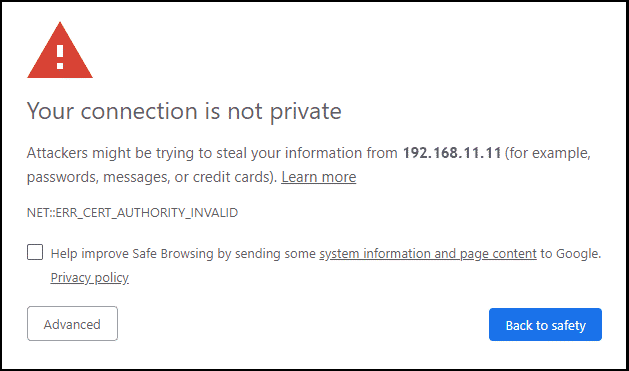
\includegraphics[width=13cm,height=9cm]{self-signed.png}
      \end{center}
      \caption{Advertencia Certificado Autofirmado}
   \end{figure}
\end{center}

Por ejemplo, para solicitar un certificado SSL de una CA de confianza como Verisign o 
GoDaddy, se debe enviar una Solicitud de firma de certificado (CSR) y te dan un 
certificado a cambio, que firmaron con su certificado raíz y clave privada. Todos 
los navegadores tienen una copia (o acceden a una copia desde el sistema operativo) 
del certificado raíz, por lo que el navegador puede verificar que su certificado 
fue firmado por una CA confiable.

Cuando generamos un certificado autofirmado, generamos nuestro propio certificado 
raíz y clave privada. Debido a que genera un certificado autofirmado, el navegador 
no confía en él. Está autofirmado. No ha sido firmado por una CA. Todos los 
certificados que generamos y firmamos serán de confianza inherente.

La principal dificultad es que los usuarios siempre encontrarán una advertencia 
donde el navegador diga que se encuentra en un sitio con un certificado autofirmado. 
En la mayoría de los casos, no verificarán que el certificado es el correcto, por 
lo que generará desconfianza en los usuarios.

En prácticamente todos los casos, un enfoque mucho mejor es utilizar una CA privada, 
que es nuestra próxima propuesta. Requiere un poco más de trabajo por adelantado, 
pero una vez que la infraestructura está establecida y la clave raíz se distribuye 
de manera segura a todos los usuarios, dichas implementaciones son tan seguras como 
el resto del ecosistema PKI.

\section{Propuesta 2: Internal CA}

Como se explicó anteriormente, una entidad de certificación es un agente en el que 
confiamos para emitir 
certificados que confirman las identidades de los suscriptores, o bien de los 
sitios a los cuales visitamos. 

Esta propuesta de solución implica establecer una entidad de certificación interna 
a la red privada, y por consiguiente hacer que los equipos que se encuentran 
dentro de la misma confíen el ella. Esto se hace 
mediante un servidor dedicado que firme los certificados que se le solicitan.

Ventajas de la autoridad de certificación interna (CA)
\begin{itemize}
   \setlength\itemsep{-0.6em}
   \item No es necesario depender de una entidad externa para los certificados.
   \item En un entorno de Microsoft Windows, la Autoridad de certificación (CA) interna se puede 
   integrar en Active Directory. Esto simplifica aún más la gestión de la estructura de la CA.
   \item No hay ningún costo por certificado cuando utiliza una Autoridad de certificación (CA) 
   interna.
\end{itemize}

Desventajas de la autoridad certificadora (CA) interna

\begin{itemize}
   \setlength\itemsep{-0.6em}
   \item Implementar una autoridad certificadora (CA) interna es más complicado que utilizar una 
   autoridad certificadora (CA) externa.
   \item La seguridad y la responsabilidad de la infraestructura de clave pública (PKI) está 
   completamente a cargo de la organización.
   \item Los usuarios externos que se conecten a nuestra red normalmente no confiarán en un 
   certificado digital 
   firmado por una Autoridad de Certificación (CA) interna.

\end{itemize}

Pese a que esta propuesta es de las más implementadas, decidimos buscar una opción que nos 
permita desligarnos de ciertas responsabilidades, como así también no tener que realizar 
configuraciones individuales a los hosts de nuestra organización. 

\subsection{Caso de estudio: Creando nuestra Entidad Certificante privada}
\subsubsection*{Servidor DNS con Docker}

Para montar esta propuesta de solución, se debió crear un servidor DNS, que lo que hace
es básicamente mapear direcciones IP a nombres de dominio. Por ejemplo: nuestra página que 
se encuentra en la dirección 192.168.0.202 se pasará a llamar pagina1.salvadorcatalfamo.intra, 
donde salvadorcatalfamo.intra abarca toda nuestra organización y las páginas que se encuentren
dentro de ella. Otra razón por la cual se debe 
crear un servidor DNS, es que los certificados no se pueden otorgar a direcciones IP, por lo 
cual es un requisito obligatorio tener las páginas web direccionadas con nombres de dominio.

Se eligió el servidor DNS CoreDNS ya que es amigable con Docker; sucede que, por cada versión del 
programa, se generan las imágenes de Docker correspondientes. Estas imágenes son públicas y oficiales, 
lo que da confiabilidad y seguridad extra a la hora de utilizarlas. La configuración está formada por 
los siguientes componentes: los archivos de configuración de CoreDNS (corefile) y los sitios que 
nosotros deseemos, en nuestro caso pagina1.salvadorcatalfamo.intra

\noindent El Corefile es el archivo de configuración de CoreDNS. Este define:
\begin{itemize}
    \setlength\itemsep{-0.6em}
    \item Que servidores escuchan en que puertos y que protocolo.
    \item Para qué zona tiene autoridad cada servidor.
    \item Que \emph{plugins} (complementos) se cargan en un servidor.
\end{itemize}

\noindent El formato es el siguiente
\begin{verbatim}
    ZONE: [PORT] {
        [PLUGIN] ...
    }
\end{verbatim}

\noindent ZONE: define la zona de este servidor. El puerto por defecto es el 53, o bien el valor que se le indique 
con el flag -dns.port.

\noindent PLUGIN: define los complementos que queremos cargar. Cada plugin puede tener varias propiedades, por 
lo que también podrían tener argumentos de entrada.

\noindent Nuestro archivo de configuración es el siguiente:
\begin{verbatim}
    .:53 {
        forward . 8.8.8.8 9.9.9.9
        log
    }

    salvadorcatalfamo.intra:53 {
        file /etc/coredns/salvadorcatalfamo
        log
        reload 10s
    }    
\end{verbatim}

A grandes rasgos, lo que indica esta configuración es que va a existir una zona 
“salvadorcatalfamo.intra”, que estará definida por el archivo que se encuentra en 
“/etc/coredns/salvadorcatalfamo”. Por otro lado, el tráfico restante (dominios externos a nuestra red)
será fordwardeado a 
servidores DNS externos (8.8.8.8 y 9.9.9.9). Además se establecieron algunos plugins de logeo y 
de refresco de configuración.

Nuestro archivo “/etc/coredns/salvadorcatalfamo” contiene la siguiente información.
\begin{verbatim}
salvadorcatalfamo.intra.          IN  SOA ns1.salvadorcatalfamo.intra. ...
pagina1.salvadorcatalfamo.intra.  IN  A   192.168.0.124   
\end{verbatim}

Esto en principio es suficiente para nuestro sitio interno, y contiene las direcciones ip de los 
servidores web y entidades certificantes.

Por el lado de Docker, se utilizó un archivo Docker-compose.yml, y un Dockerfile. 
Docker-compose es una herramienta para definir y ejecutar aplicaciones Docker de 
varios contenedores. Compose usa un archivo YAML para configurar los servicios de 
la aplicación. Luego, con un solo comando, se crean e inician todos los servicios 
desde este archivo de configuración. En nuestro caso, se definió de la siguiente 
manera

\begin{verbatim}
version: `3.1'
services:
    coredns:
        build: .
        container_name: coredns
        restart: always
        expose:
            - `53'
            - `53/udp'
        ports:
            - `53:53'
            - `53:53/udp'
        volumes:
            - `./config:/etc/coredns'    
\end{verbatim}

\noindent Por otro lado, el fichero dockerfile está compuesto por las siguientes líneas:
\begin{verbatim}
FROM coredns/coredns:1.7.0
ENTRYPOINT ["/coredns"]
CMD ["-conf", "/etc/coredns/Corefile"]    
\end{verbatim}

En conjunto, establecen la imagen de CoreDNS que se utilizará, los archivos de configuración y
los puertos que se expondrán, entre otras configuraciones.

\subsubsection*{Creación de nuestra CA en Docker}

La estrategia para crear nuestra CA será seguir los pasos que se deberían realizar en un servidor 
habitual, pero partiendo desde una imagen de Docker de Ubuntu (de stock), y luego realizando un 
commit de estas configuraciones. Luego, archivos importantes como el certificado root y la llave
privada deberán resguardarse, o simplemente resguardar el contenedor creado. 

Se utilizó esta estrategia ya que no había imágenes oficiales que nos sirva para tal fin, por el 
simple hecho de que únicamente se requiere tener instalado OpenSSL y tenerlo configurado.

\noindent Como primer paso, corremos una imagen del sistema operativo Ubuntu

\begin{verbatim}
    docker run -it -v $PWD/ca:/root/ca ubuntu
\end{verbatim}

\noindent Dentro del contenedor, ejecutamos los siguientes comandos:
\begin{verbatim}
    apt-get update
    apt-get install ntp
    apt-get install openssl
\end{verbatim}

\noindent Establecer el hostname al contenedor, hay una línea con la ip del contenedor y el nombre del mismo, 
que es utilizado como hostname, en nuestro caso
\begin{verbatim}
    172.17.0.2      080dec560726
\end{verbatim}

\noindent Lo cambiamos por un hostname con el dominio incluido
\begin{verbatim}
    172.17.0.2      ca.salvadorcatalfamo.intra
\end{verbatim}

\noindent Creamos las carpetas para mejor organización
\begin{verbatim}
    mkdir /root/newcerts
    mkdir /root/certs
    mkdir /root/crl
    mkdir /root/private
    mkdir /root/requests
\end{verbatim}

\noindent Creamos un archivo vacío y un archivo que contiene el primer número de serie para los certificados 
\begin{verbatim}
    touch index.txt
    echo '1234' > serial
\end{verbatim}

\noindent Luego hay que crear la llave privada y el certificado root, en este caso nos pedirá una contraseña, si este servidor 
se usará en un ambiente de producción, deberá ser una contraseña compleja.

\begin{verbatim}
    openssl genrsa -aes256 -out private/cakey.pem

\end{verbatim}

\noindent Una vez que generamos la llave privada, la misma será utilizada como entrada en la creación de 
nuestro certificado root. Nos pedirá algunos datos de localización y relacionados a la 
organización

\begin{verbatim}
    openssl req -new -x509 -key /root/ca/private/cakey.pem 
            -out cacert.pem -days 3650
\end{verbatim}

\noindent Cambiamos los permisos de los archivos que creamos
\begin{verbatim}
    chmod 600 -R /root/ca
\end{verbatim}

\noindent Realizamos unas modificaciones en el archivo de configuración, donde indicaremos 
la dirección de los certificados, y algunas opciones de configuración adicionales
\begin{verbatim}
    vim /usr/lib/ssl/openssl.cnf
\end{verbatim}

Una vez que realizamos estos pasos, estamos listos para realizar el commit de la imagen, con esto,
todos los pasos que realizamos (instalar los paquetes, modificar los archivos de configuración, etc)
no son necesarios que se ejecuten nuevamente.

Para realizar un commit, y que nuestro contenedor sea fácilmente identificable, deberemos seguir 
los siguientes pasos

\begin{verbatim}
    docker ps -a        #identificamos el último contenedor utilizado
    docker commit {id_del_contenedor} 
    docker image ls     #Identificamos la imagen recién creada
                        #no tendrá ni repositorio ni tag
    docker image tag {id_de_imagen} ca:1.0  #nombramos nuestra imagen
\end{verbatim}




Ahora cada vez que queramos correr nuestra CA, lo haremos de la siguiente manera:
\begin{verbatim}
    docker run -it -v $PWD/ca:/root/ca ca:1.0
\end{verbatim}

Em el comando anterior, estamos asumiendo que queremos compartir los archivos de la CA con el servidor 
host.

 

\subsubsection*{Nginx con Docker}

Para probar nuestro certificado, utilizaremos una imagen oficial de Nginx, 
los archivos de configuración
son los siguientes:


\begin{verbatim}
docker-compose.yml

web:
  image: nginx
  volumes:
   - ./pagina1:/usr/share/nginx/html:ro
  ports:
   - "80:80"
  environment:
   - NGINX_HOST=pagina1.salvadorcatalfamo.intra
   - NGINX_PORT=80
\end{verbatim}

En el archivo mostrado, le decimos a Docker que utilice la imagen Nginx, 
que nuestros archivos fuentes
van a estar en el directorio \textit{./pagina1} y que exponga el puerto 80, entre otras
 cosas.

\noindent Para ejecutar este contenedor, se debe ejecutar el siguiente comando:

\begin{verbatim}
    docker-compose up -d
\end{verbatim}




\subsubsection*{Creando nuestro certificado}

Para firmar un certificado, tenemos que seguir los pasos mostrados en la figura \ref{figSolCert}
: el servidor donde se alojará la web debe realizar una solicitud, 
luego nuestra CA retornará el certificado firmado. Desde el servidor web en cuestión, se debe 
crear una llave privada:

\begin{verbatim}
    openssl genrsa -aes256 -out pagina1.pem 2048
\end{verbatim}

\noindent Luego, se deberá crear la solicitud de firma de certificado:
\begin{verbatim}
    openssl req -new -key pagina1.pem -out pagina1.csr
\end{verbatim}

\noindent Luego enviamos esta solicitud y la firmamos en nuestra CA, esta solicitud la vamos a colocar 
en el directorio \textit{/root/ca/requests}
\begin{verbatim}
    openssl ca -in pagina1.csr -out pagina1.crt
\end{verbatim}

\subsubsection*{Configuración del certificado en el servidor web}
Una vez que tenemos este certificado, lo colocamos en el servidor web y 
lo configuramos. Para el caso de Nginx, se debe editar el archivo de configuración 
correspondiente a nuestra web, que en este caso es \textit{pagina1.salvadorcatalfamo.intra}
con el fin de que el mismo pueda localizar correctamente los certificados firmados recientemente.
Adicionalmente, se puede obligar a que cada requerimiento sea redirigido a una conexión
segura mediante SSL.

Como se puede ver en la figura \ref{figCAdesc}, aunque el certificado esté configurado, 
el mismo no es confiable ya que nuestra entidad certificante no está importada a nuestro almacén 
local.

\begin{center}
    \begin{figure}   
       \begin{center}
          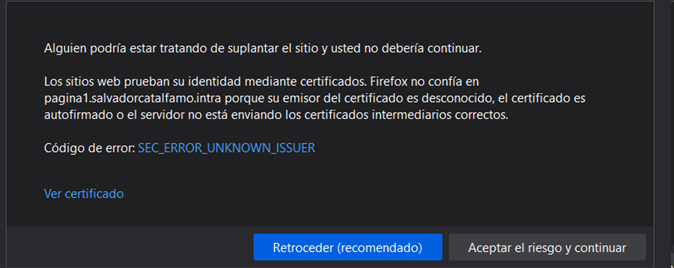
\includegraphics[width=15cm,height=6cm]{adv-2.png}
       \end{center}
       \caption{CA Desconocida}
       \label{figCAdesc}
    \end{figure}
 \end{center}

Luego de establecer en nuestra computadora (particularmente en el navegador Mozilla) que la 
entidad certificante creada es confiable, es posible ver que nuestra conexión es segura, como 
se muestra en la captura.

\begin{center}
    \begin{figure}   
       \begin{center}
          \includegraphics[width=15cm,height=7.5cm]{ca-HTTPS.png}
       \end{center}
       \caption{Resultado de la solución}
    \end{figure}
 \end{center}







\section{Propuesta 3: Certificación con Let's Encrypt}
Esta estrategia consiste en generar un certificado wildcard, y utilizarlo en cada sitio de la organización.
Para esto se debe tener un dominio (en mi caso, salvadorcatalfamo.com) y demostrar la propiedad 
del mismo. Como se vio anteriormente, hay dos maneras que utiliza Let's Encrypt para demostrar la propiedad 
de un dominio, pero la que nos sirve en el caso de una red interna es la que intervienen los registros DNS. 
La verificación que ofrecen con este tipo de certificado es la mínima (DV) y el proceso es explicado a 
continuación.


\subsection{Pasos a seguir}
\subsubsection*{Obtener un dominio}
El primer paso es conseguir un dominio, en mi caso ya tenía uno:
salvadorcatalfamo.com. Este dominio apunta a nuestra ip pública. La configuración DNS
es la siguiente:  


\begin{longtable}{|l|l|p{5cm}|l|l|} 
   \hline
   \textbf{Tipo} & \textbf{Nombre} & \textbf{Contenido} & \textbf{Prioridad} & \textbf{TTL}
\\ \hline A  & salvadorcatalfamo.com & 181.228.121.12 & 0 & 14400
\\ \hline NS  & salvadorcatalfamo.com & ns1.donweb.com & 0 & 14400
\\ \hline SOA & salvadorcatalfamo.com & ns2.donweb.com & 0 & 14400
\\ \hline SOA & salvadorcatalfamo.com & ns3.hostmar.com \newline root.hostmar.com 
                                       \newline 2021010700 28800 7200 
                                       \newline 2000000 86400
                                       \newline ns2.donweb.com & 0 & 14400                  


\\ \hline
\end{longtable}

\subsubsection*{Instalando Let’s Encrypt en el servidor}
\begin{verbatim}
   sudo add-apt-repository ppa:certbot/certbotsudo 
   apt-get update
   sudo apt-get install python-certbot-nginx
\end{verbatim}

\subsubsection*{Instalando Nginx}
\begin{verbatim}
sudo apt-get update
sudo apt-get install nginx
\end{verbatim}


\subsubsection*{Obteniendo un certificado SSL de tipo wildcard desde Let’s Encrypt}
\begin{verbatim}
sudo certbot --server https://acme-v02.api.letsencrypt.org/directory 
-d *.salvadorcatalfamo.com --manual --preferred-challenges dns-01 certonly
\end{verbatim}

\subsubsection*{Configuración DNS}
Luego de ejecutar el comando anterior, Let's Encrypt nos da un contenido que 
se debe agregar a un registro DNS. El tipo de registro es TXT y se muestra en
la siguiente tabla.

\begin{longtable}{|l|l|l|l|l|} 
   \hline
   \textbf{Tipo} & \textbf{Nombre} & \textbf{Contenido} & \textbf{Prioridad} & \textbf{TTL}
\\ \hline TXT  & 	\_acme-challenge.salvadorcatalfamo.com & 11UZJD27bPDb\_jFs6f... & 0 & 14400
\\ \hline
\end{longtable}

\subsubsection*{Configuración de Nginx para servir a subdominios}

Se debe modificar el siguiente archivo de 
configuración 

/etc/nginx/sites-available/salvadorcatalfamo.com como se muestra a 
continuación:

\begin{verbatim}
server {
   listen 80;
   listen [::]:80;
   server_name *.salvadorcatalfamo.com;
   return 301 https://$host$request_uri;
}
server {
   listen 443 ssl;
   server_name *.example.com;  ssl_certificate /.../.../fullchain.pem;
   ssl_certificate_key /.../privkey.pem;
   include /etc/letsencrypt/options-ssl-nginx.conf;
   ssl_dhparam /.../ssl-dhparams.pem;  root /.../salvadorcatalfamo.com;
   index index.html;
   location / {
      try_files $uri $uri/ =404;
   }
} 
\end{verbatim}


\subsubsection*{Test la configuración y reinicio del servicio}

La configuración se puede testear con el siguiente comando: 
\begin{verbatim}
      sudo nginx -t
\end{verbatim}

Si tiene éxito, se debe volver a cargar Nginx usando
\begin{verbatim}
      sudo /etc/init.d/nginx reload
\end{verbatim}

Ahora Nginx contiene un certificado de tipo wildcard, un certificado SSL con respaldo de una 
entidad certificante como Let's Encrypt

\begin{center}
   \begin{figure}   
      \begin{center}
         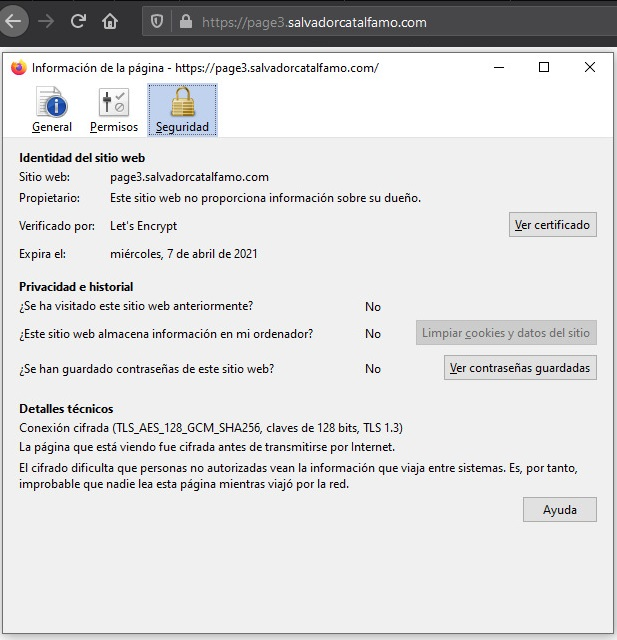
\includegraphics[width=15cm,height=16cm]{lets.png}
      \end{center}
      \caption{Web interna con certificado de Let’s Encrypt}
   \end{figure}
\end{center}

Le hemos visto un gran potencial a esta solución, aunque también es poco implementada. Tenemos la gran ventaja de no
tener que instalar ningún requerimiento en las computadoras dentro de la organización. Con esto, no se 
mostrarán mensajes de seguridad en los navegadores, no importa cuál sea el programa, ya que Let's Encrypt es 
una entidad de confianza para diversos navegadores y sistemas operativos. Todo esto y la seguridad extra al 
saber que nuestros datos van por un canal seguro gracias al protocolo SSL. 

Otra gran ventaja que vimos es la facilidad con la que se llevó a cabo, 
en este proyecto se logró implementar antes esta solución que la entidad certificante, y 
con mucha mayor facilidad. 

Como desventajas podemos decir que no tenemos la posibilidad de obtener la validación extendida (EV), ya que no está
disponible actualmente. Por otro lado, que las llaves privadas y el certificado (que es único para todo el dominio) 
estén en diversos servidores a la vez, implica
que se deben tener mayores recaudos a la hora de utilizarlos, ya que se debe asegurar el control de éstos. Aunque a 
nosotros no nos sucedió, puede llegar a suceder que si se pierde conexión a Internet, el certificado no se pueda validar,
producto de no tener toda la cadena de certificación hasta llegar a la raíz. 

Aunque se puede llegar a pensar, administrar los certificados y las llaves puede llegar a ser 
un gran desafío para los administradores de sistema, sin embargo, hay muchas herramientas que nos proveen
automatización y monitoreo para realizar esta clase de tareas. 


\section{Caso de estudio: Buscando credenciales en tráfico seguro}

Luego de ver las diversas soluciones propuestas, una parte importante de 
nuestro proyecto fue verificar que verdaderamente aumenta la seguridad
cuando nuestro tráfico va encriptado. Para este caso de estudio, se utilizó
el mismo formulario propuesto en la sección \ref{secCaseOfStudy}, lo 
único que con servidores en distintas direcciones.

Dado que el proceso de capturar el tráfico en una red interna fue
explicado previamente, se van a mostrar únicamente los paquetes capturados
desde la primera solicitud hasta el envío del formulario.

\begin{center}
   \begin{figure}   
      \begin{center}
         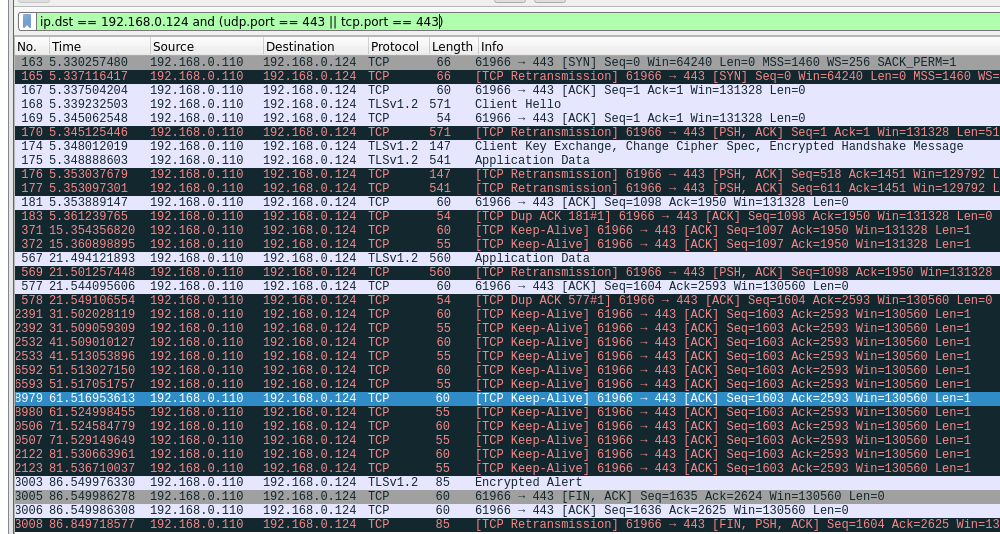
\includegraphics[width=15cm,height=9cm]{verificacion-ssl-1-v2.png}
      \end{center}
      \caption{Tráfico capturado}
   \end{figure}
\end{center}

En esta captura podemos observar que:
\begin{itemize}
   \setlength\itemsep{-0.6em}
   \item No es posible determinar a simple vista cual es el paquete 
   en el cual se envía la información crítica.
   \item Abriendo e investigando el contenido de cada uno de los paquetes mostrados,
   tampoco es posible ver las credenciales completadas en el formulario, 
   que obviamente son de nuestro conocimiento.
   \item Se establece una conexión segura a través del protocolo TCP, algo que no 
   vimos en el caso de estudio de HTTP.
\end{itemize}





% =================================================================== %

\chapter{Conclusiones y Resultados Obtenidos}
    \label{capConc}

%-*- ES -*-
%----------------------------------------------------------------------
% Capitulo 7: Conclusiones generales
%----------------------------------------------------------------------

En este proyecto abordamos una amplia cantidad de temas de manera resumida, con un gran potencial 
de estudio por delante. Aunque en un principio se deseaba investigar todo el tráfico que pasaba por 
la red interna, con todas las posibles debilidades, la navegación web nos permitió encontrar una 
extensa cantidad de nuevos conceptos para desarrollar, tales como los protocolos HTTP, HTTPS, DNS, 
y los posibles procesos que se pueden realizar para segurizar nuestra red.

Con respecto a Docker, no nos resultó muy complejo realizar nuestras tareas, ya que la comunidad 
es muy amplia, y las herramientas que nos brindan están al alcance de nuestra mano. El tiempo que 
nos ahorramos con Docker fue destinado a entender el funcionamiento de la seguridad en las redes, 
tales como el uso de los certificados SSL y las entidades certificantes.

A pesar del contenido teórico propuesto, el trabajo se concentró en las soluciones presentadas 
en el capítulo 4. Allí se explicó brevemente como con un corto conocimiento en el funcionamiento 
del protocolo SSL se pueden establecer mecanismos para que el tráfico web vaya de manera segura; 
uno de nuestros principales objetivos, junto con el de concientizar a las personas de la 
importancia de conocer los sitios por los que se navega. Aunque en nuestro caso abordamos las 
redes pertenecientes a una organización, el contenido de la información es válido para cualquier 
sitio web que se visita, ya sea interno o externo. 


% =================================================================== %

\appendix
\chapter{Glosario}

%-*- ES -*-
\section{Terminolog\'{\i}a}

\begin{longtable}{|l|l|} \hline
\textbf{T\'ermino en ingl\'es} & \textbf{Traducci\'on utilizada}
\\ \hline \hline stateless & sin estado
\\ \hline Secure Sockets Layer & capa de Sockets seguros
\\ \hline wildcard & comodín
\\ \hline framework & sistema
\\ \hline man-in-the-middle & hombre en el medio
\\ \hline Sniffing & olfateo
\\ \hline Spoofing & engañar
\\ \hline Self-signed Certificates & certificados auto-firmados
\\ \hline Namespaces & espacios de nombres  \\ \hline
\end{longtable}




%bibliografia
\bibliography{tesis}
\bibliographystyle{acm}
%\bibliographystyle{alpha}


\end{document}
